\section{问题分析}

\subsection{问题一分析}

问题一属于确定性功率平衡计算问题。在电解槽与合成氨装置满负荷连续运行的前提下，园区每时段的制氢氨负荷功率为固定值（ALKEL 10~MW + PEMEL 10~MW + 合成氨 0.75~MW = 20.75~MW），加上随时间变化的常规电负荷，构成总用电需求。风光发电功率由附件2的标幺功率曲线乘以装机容量确定。根据功率平衡原则，当新能源发电超过负荷时余电上网，不足时从电网购电。核心难点在于风光出力的时序分布与负荷需求的时序匹配程度直接决定了绿电直连指标的达标情况。

\subsection{问题二分析}

问题二是一个组合优化问题。产能扩至72吨/日后，设备功率线性扩容至2倍（制氢氨总负荷41.5~MW）。制氨产量从72吨/日按9吨递减至36吨/日，对应运行时段从24小时递减至12小时。由于电氢氨装置只有全额开机和停机两种方式，问题转化为从24个时段中选择$h$个时段开机的0-1整数规划问题。目标函数为吨氨成本最小化，其中购电成本受分时电价影响，售电收入与风光余电量相关。由于每时段的开机边际成本可独立计算，贪心策略等价于整数线性规划的精确解。

\subsection{问题三分析}

问题三将离散调节放宽为连续调节，电氢氨装置功率可在额定值的10\%至100\%之间连续变化。决策变量从0-1整数变量变为连续出力系数$\alpha(t) \in [0.1, 1]$（或停机时$\alpha(t)=0$），可行域从离散组合扩展为连续凸集。这使得制氢氨负荷能够更精细地跟踪风光出力波动，减少购电需求和弃电量。问题转化为以24个时段出力系数为决策变量的线性规划问题，约束包括产量等式约束和功率平衡约束。

\subsection{问题四分析}

问题四研究园区离网运行场景，即切断与外部电网的连接，园区用能完全依赖风光发电。无储能时，每时段的制氢氨负荷受限于当时的风光可用功率，产量取决于风光资源的时序分布。引入储能后，可将风光富余时段的电能储存并在不足时段释放，实现时间维度上的能量转移\cite{ref8,ref9}。储能配置优化是一个两层问题：外层搜索最优储能容量，内层在给定容量下求解含储能的最优调度方案\cite{ref6}。最终需对比离网（有储能）与联网两种模式的全年经济性。

\begin{figure}[H]
\centering
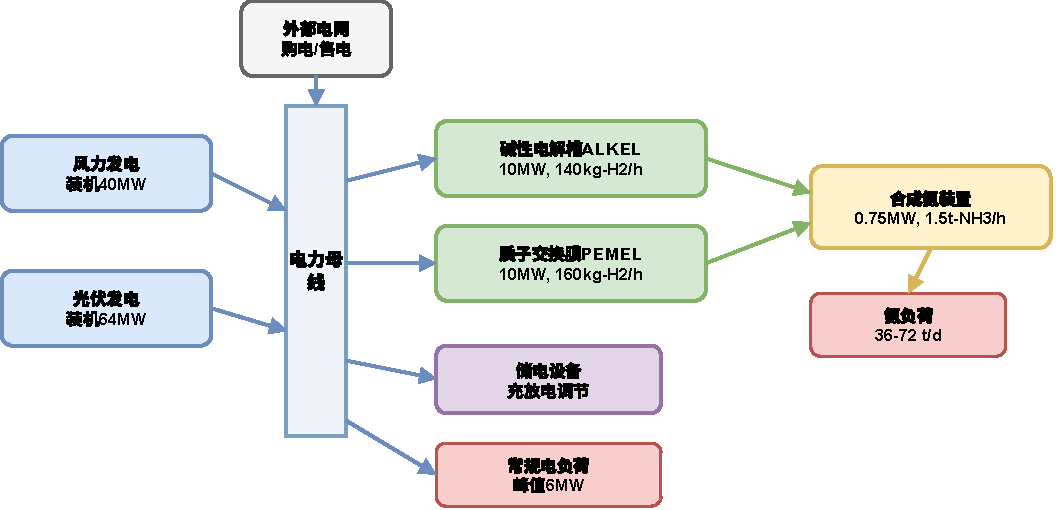
\includegraphics[width=0.9\textwidth,height=0.3\textheight,keepaspectratio]{../figures/fig_system_arch.pdf}
\caption{绿电直连型电氢氨园区系统架构}\label{fig:system_arch}
\end{figure}

综合来看，四个问题呈递进关系：问题一建立基准模型，问题二引入离散优化，问题三扩展为连续优化，问题四进一步考虑离网和储能配置。园区系统架构如图\ref{fig:system_arch}所示，风电和光伏通过内部母线为电解槽、合成氨装置和常规电负荷供电，储能设备实现充放电调节，外部电网提供购售电通道。
